\chapter{Resultados detallados}

Este capítulo presenta una evaluación exhaustiva del rendimiento de los sistemas de ficheros ext4, Btrfs, XFS y ZFS bajo una serie de condiciones de prueba específicas. 

\section{Pruebas de lectura}

\subsection{Lectura}

En la prueba de lectura secuencial, podemos apreciar cómo Btrfs obtiene un rendimiento excelente para tamaños de fichero muy pequeños, entre 4 kB y 65 kB, incluso cuadruplicando el rendimiento de los demás sistemas de ficheros comparados. Este comportamiento se fundamenta en su estructura arborescente, así como en la subasignación de bloques. Btrfs implementa una subasignación de bloques que permite manejar eficientemente archivos pequeños. En Btrfs, los bloques se pueden dividir en sub-bloques más pequeños, y múltiples archivos pequeños pueden ocupar diferentes sub-bloques dentro del mismo bloque. Esto reduce el espacio desperdiciado y permite que el sistema de ficheros mantenga una alta densidad de datos. Como resultado, cuando el sistema necesita acceder a un archivo pequeño, puede localizarlo y cargarlo rápidamente desde el bloque contiguo, mejorando el rendimiento.\\

También apreciamos cómo en Btrfs, puesto que el tamaño de bloque elegido para la prueba es de 8 kB, el rendimiento de este sistema de ficheros aumenta hasta llegar a 8 kB de tamaño de fichero. Esto se debe a la lectura multisector, que se refiere a la capacidad del sistema de leer múltiples sectores consecutivos del disco en una sola operación. Esta aceleración producida por la lectura multisector se va perdiendo una vez superado el tamaño de bloque, lo que se puede ver reflejado a partir de los 8 kB de tamaño de fichero. \\

\newpage

\begin{figure}[h!]
    \centering
    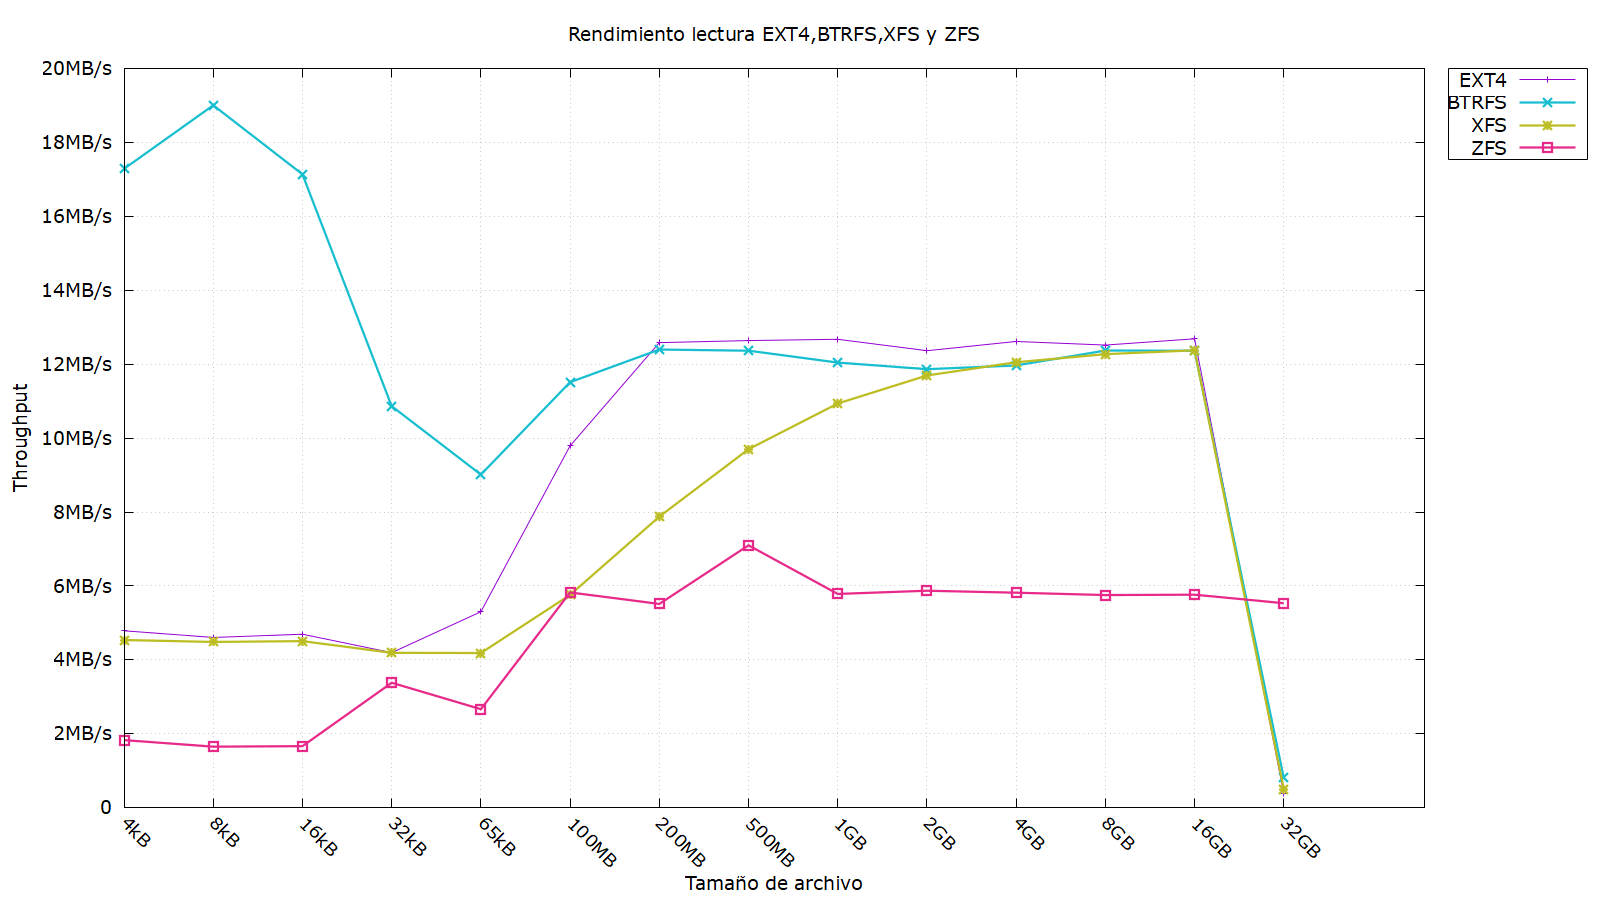
\includegraphics[width=1\linewidth]{results/read_throughput_plot.png}
    \caption{Rendimiento de lectura de ext4, Btrfs, XFS y ZFS en MB/s}
    \label{fig:lectura_throughput}
\end{figure}

Podemos apreciar también cómo, conforme aumenta el tamaño del fichero, aumenta el throughput obtenido, llegando al punto máximo de la controladora. Este punto máximo indica el máximo de bytes por segundo que el disco puede suministrar al sistema operativo en ese momento. Este punto está en torno a los 12 MB/s, y podemos ver cómo ext4 y Btrfs alcanzan este rendimiento al mismo tiempo, alrededor de los 200 MB de tamaño de fichero. XFS, en cambio, obtiene el rendimiento máximo de la controladora en torno a los 8 GB de tamaño de archivo. \\

\begin{table}[h!]
\centering
\caption{Rendimiento de lectura de ext4, Btrfs, XFS y ZFS en MB/s}
\begin{tabular}{|l|c|c|c|c|}
\hline
\textbf{Métrica} & \textbf{ext4} & \textbf{Btrfs} & \textbf{XFS} & \textbf{ZFS} \\ \hline
Mínimo           & 0,38 MB/s     & 0,80 MB/s      & 0,50 MB/s    & 5,53 MB/s \\ \hline
Máximo           & 12,69 MB/s    & 19,01 MB/s     & 12,38 MB/s   & 7,75 MB/s \\ \hline
Promedio         & 8,70 MB/s     & 12,21 MB/s     & 7,50 MB/s    & 4,58 MB/s \\ \hline
Desviación Típica & 4,44 MB/s     & 4,29 MB/s      & 3,95 MB/s    & 1,90 MB/s \\ \hline
\end{tabular}
\label{tab:rendimiento_lectura_sistemas_archivos}
\end{table}

ZFS, por su parte, no llega a alcanzar el rendimiento máximo de la controladora del disco. Esto se debe a la lógica detrás del propio sistema de ficheros, viéndose afectado por las técnicas de integridad como los checksums. Estos no solo se aplican en las operaciones de escritura; de hecho, cuando se solicitan leer datos del disco en el caso de ZFS, antes de devolver los datos a la aplicación, ZFS necesita calcular el checksum que da integridad al bloque, y una vez calculado, necesita ser comparado con el checksum almacenado en sus metadatos. \\

Podríamos pensar que las cachés agilizarían estas lecturas, pero esta aceleración no es tan significativa como en los demás sistemas de ficheros. Incluso en el caso de que los datos solicitados estén en la caché, ZFS aún realiza una verificación del checksum para asegurarse de que los datos en la memoria no estén corruptos. \\

Hemos observado, además, cómo la caché del sistema, que en este caso era de 32 GB, solo llegaba a dedicar 16 GB para el buffer caché y la caché de páginas. Es decir, aun teniendo espacio disponible para almacenar bloques de disco en memoria, el máximo que permitía aumentar esa caché el sistema operativo era de 16 GB. Aunque este parámetro puede ser modificado cambiando configuraciones del kernel, por lo general este tipo de caché se suele limitar a la mitad del tamaño total de memoria RAM del equipo. \\

Podemos apreciar también cómo los tres sistemas de ficheros que llegan al máximo rendimiento de la controladora, ext4, Btrfs y XFS, y que, por tanto, llenan la caché con bloques de disco, sufren una caída de rendimiento en el salto de 16 GB a 32 GB. Esto se debe a la necesidad de traer nuevos bloques de disco a la caché y a su vez desalojar otros por falta de espacio. Además, el hecho de generar un gran número de solicitudes de lectura simultáneas para traer esos bloques faltantes hace que se sature la cola de la controladora de disco, reduciendo el rendimiento significativamente en la marca de 32 GB de tamaño de fichero. \\

Cabría esperar que la caída del rendimiento de ZFS se produjese más adelante, quizá en el salto de 32 GB a 64 GB, pero el análisis de este escenario implica una carga de trabajo que sería más apropiada para una tesis doctoral y de una forma más detallada que el trabajo de fin de grado.

\subsection{Relectura}

En el caso de la relectura, podemos apreciar cómo nuevamente Btrfs se beneficia de un rendimiento que triplica para tamaños de fichero muy pequeños, desde 4 kB hasta 32 kB. Una vez pasado este umbral, el rendimiento se estabiliza y se alcanza el máximo rendimiento de la controladora para este sistema de ficheros.\\

Específicamente, Btrfs alcanza el rendimiento máximo de la controladora con archivos de apenas 32 kB, antes incluso que en la prueba de lectura secuencial, donde se alcanzaba con archivos de 200 MB. Mientras tanto, ext4 y XFS logran este pico con archivos cercanos a los 100 MB, ligeramente antes que en la prueba de lectura secuencial. Este fenómeno se presenta mucho antes en la relectura debido al uso efectivo de las cachés, cuyo impacto es tan significativo que los sistemas ext4, XFS y Btrfs muestran un rendimiento prácticamente idéntico a partir de los 100 MB de tamaño de fichero. El pico de rendimiento de la controladora, que asciende a 12 MB/s, es consistente con los observados en las pruebas de lectura secuencial.\\

Una vez más, se observa que las cachés pierden efectividad cuando el tamaño del archivo supera los 16 GB, resultando en una abrupta caída del rendimiento al escalar hasta los 32 GB. Esto se debe a la necesidad de desalojar páginas de la memoria caché para alojar otras nuevas, produciendo fallos al traer bloques de disco a memoria y penalizando el rendimiento, que disminuye hasta prácticamente 1 MB/s.\\

Al igual que en la prueba de lectura secuencial, ZFS muestra un rendimiento considerablemente menor en comparación con otros sistemas de ficheros debido a su cifrado y sus métodos de respaldo. Sin embargo, destaca por no experimentar una caída pronunciada en el rendimiento al pasar de archivos de 16 GB a 32 GB. Esto se debe a que, al no agotar el tamaño de la caché, aún tiene margen para almacenar en ella bloques de disco. Podemos suponer que este sistema alcanzaría su punto más bajo en saltos superiores a los 32 GB, probablemente en el de 32 GB a 64 GB de tamaño de archivo.\\

\begin{figure}[h!]
    \centering
    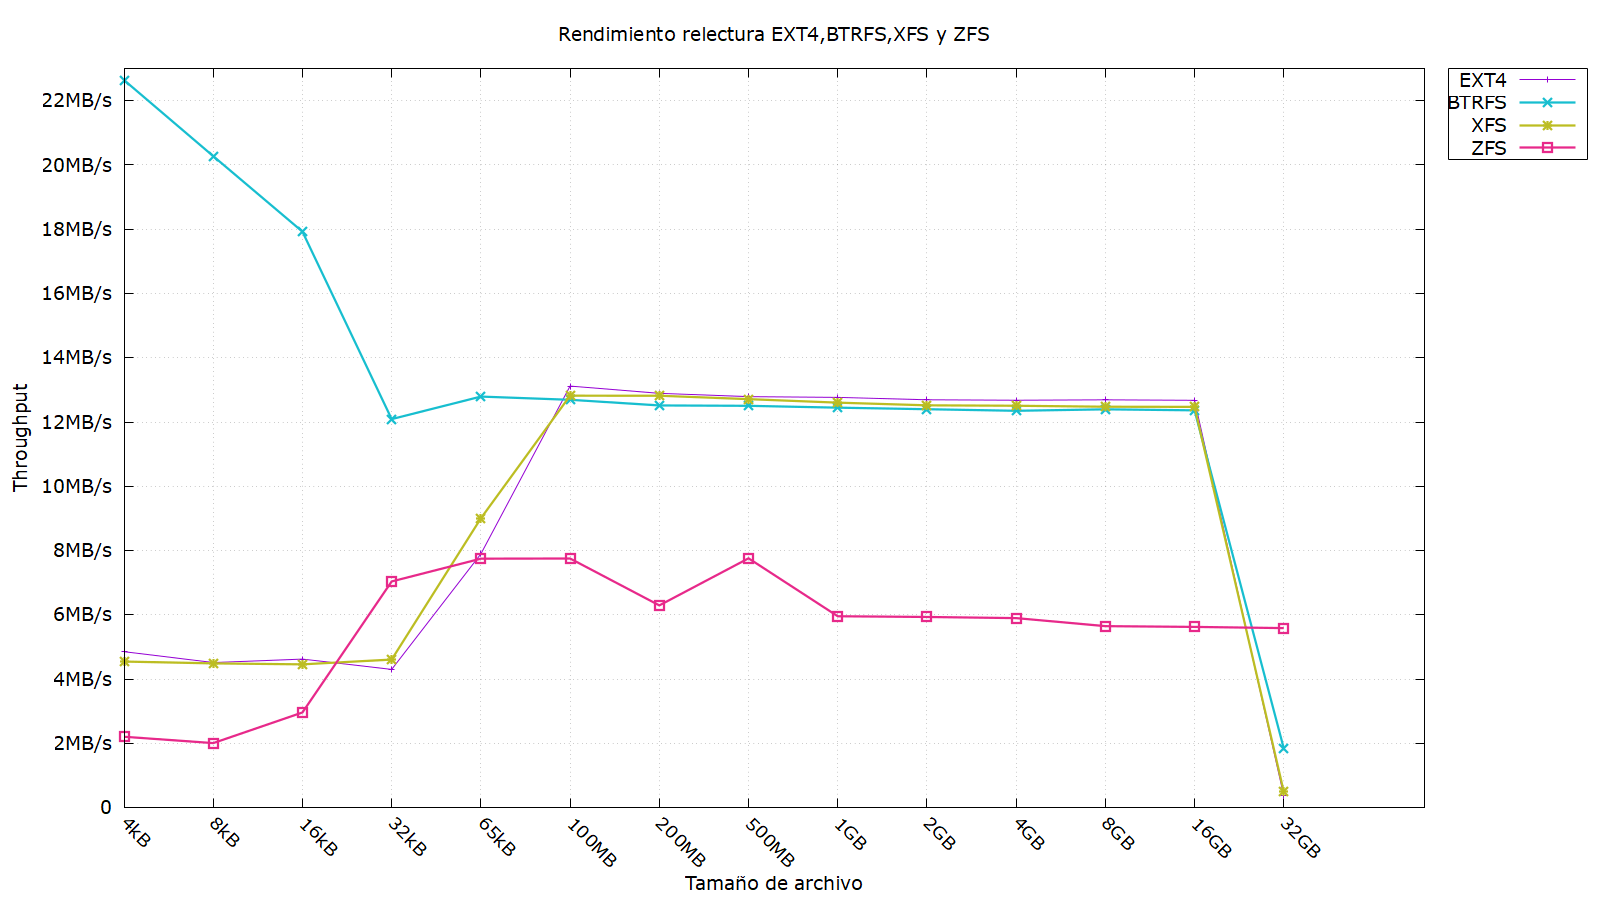
\includegraphics[width=1\linewidth]{results/reread_throughput_plot.png}
    \caption{Rendimiento de relectura de ext4, Btrfs, XFS y ZFS en MB/s}
    \label{fig:relectura_throughput}
\end{figure}

\begin{table}[h!]
\centering
\caption{Rendimiento de relectura de ext4, Btrfs, XFS y ZFS en MB/s}
\begin{tabular}{|l|c|c|c|c|}
\hline
\textbf{Métrica} & \textbf{ext4} & \textbf{Btrfs} & \textbf{XFS} & \textbf{ZFS} \\ \hline
Mínimo           & 0,37 MB/s     & 1,85 MB/s      & 0,50 MB/s    & 5,59 MB/s \\ \hline
Máximo           & 12,69 MB/s    & 22,64 MB/s     & 12,82 MB/s   & 7,75 MB/s \\ \hline
Promedio         & 9,20 MB/s     & 13,37 MB/s     & 9,18 MB/s    & 5,60 MB/s \\ \hline
Desviación Típica & 4,55 MB/s     & 4,77 MB/s      & 4,44 MB/s    & 1,92 MB/s \\ \hline
\end{tabular}
\label{tab:rendimiento_relectura_sistemas_archivos}
\end{table}

\subsection{Lectura estratificada}

Una vez más, debido al tamaño de bloque seleccionado en las pruebas, vemos cómo se repite el caso en el que hasta los 8 kB de tamaño de fichero, el rendimiento de Btrfs va subiendo. Esto, como ya hemos comentado en las gráficas de lecturas previas, se debe a la lectura multisector. \\

En la prueba de lectura estratificada, observamos que el rendimiento máximo del sistema en el caso de Btrfs se alcanza con archivos de aproximadamente 32 kB, beneficiándose nuevamente de la subasignación de bloques. A partir de ese momento, la caché comienza a actuar de forma significativa y provoca una aceleración en cada uno de los sistemas de archivos. \\

Dado que esta prueba lee con un comportamiento escalonado, el rendimiento pico se alcanza antes que en las demás lecturas, fomentando la aceleración del caché debido a un mayor número de aciertos en la memoria. En lugar de leer datos de manera secuencial, el acceso escalonado lee bloques de datos de forma discontinua. Por ejemplo, el programa puede leer un bloque de datos, saltar varios bloques, leer otro bloque, y así sucesivamente. Si el tamaño del bloque es de 4 KB y el stride es de 16 KB, Iozone leerá 4 KB, luego saltará 16 KB, leerá los siguientes 4 KB, y así sucesivamente. \\

De este modo, a partir de los 65 kB, ext4, Btrfs y XFS muestran una estabilización en el pico de rendimiento, limitándose entonces a la máxima capacidad que la controladora puede ofrecer en esos momentos. A diferencia de las pruebas de lectura anteriores, y debido a la naturaleza no secuencial de la prueba, ZFS presenta un descenso en el rendimiento al pasar del tamaño de fichero de 500 MB a 1 GB, y estabilizándose a partir de ese momento. Esto se puede deber a los mecanismos internos de implementación de ZFS, ya que, por lo que intuimos, la compresión y actualización de los metadatos a partir de estos tamaños penaliza gravemente el rendimiento del sistema de ficheros. Es por esto que el rendimiento a partir de 1 GB de tamaño de archivo se estabiliza. \\

\begin{figure}[h!]
    \centering
    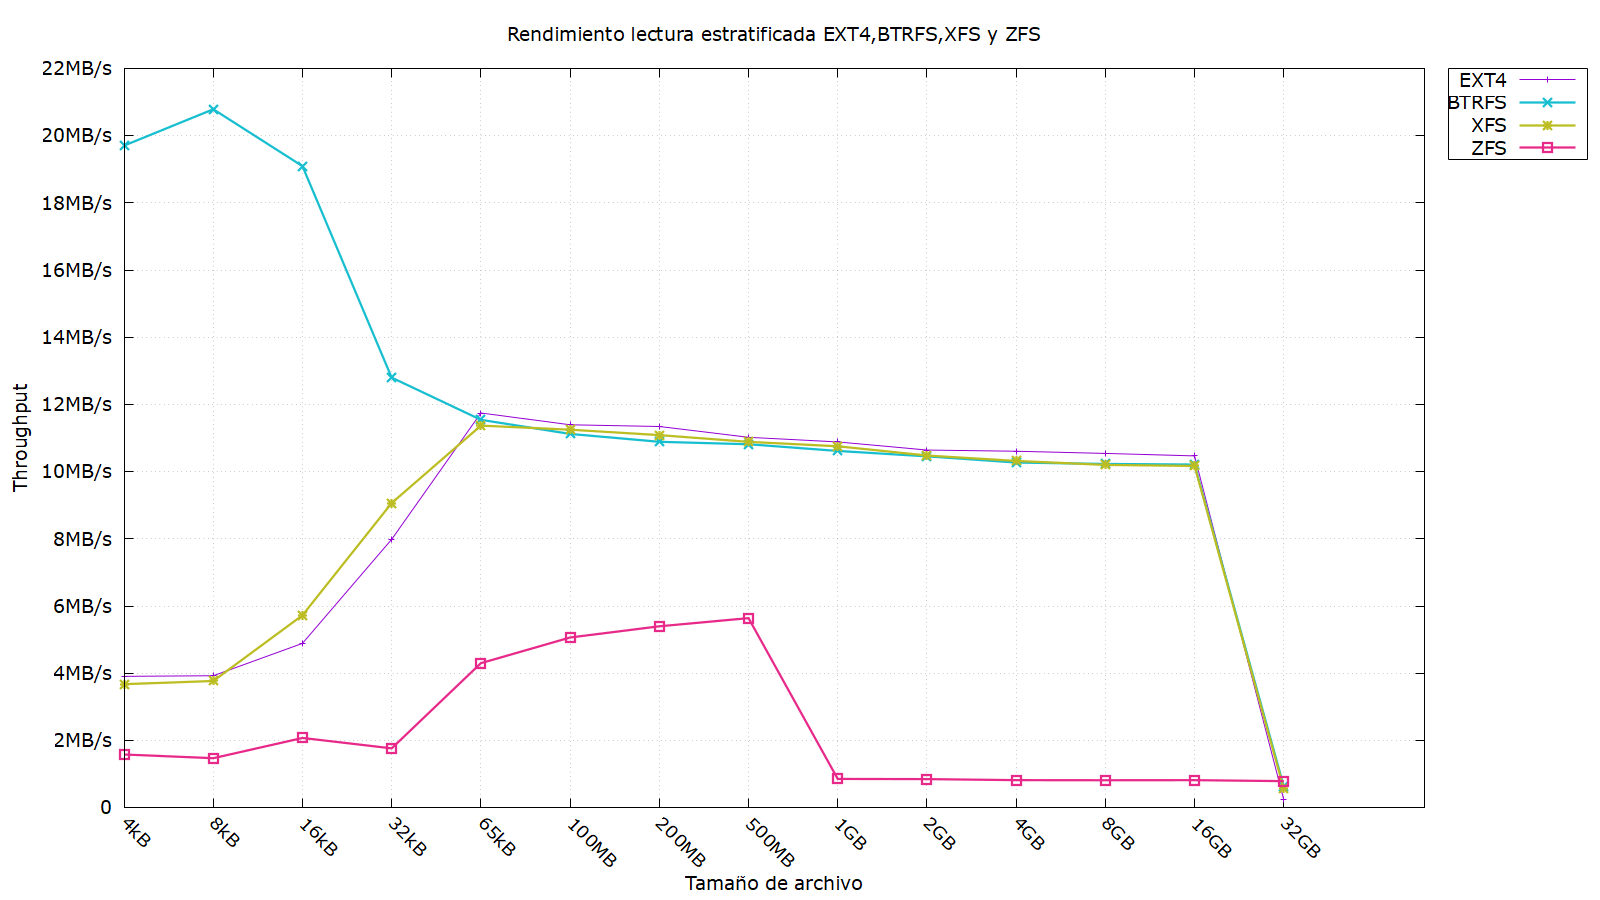
\includegraphics[width=1\linewidth]{results/strided_read_throughput_plot.png}
    \caption{Rendimiento de lectura estratificada de ext4, Btrfs, XFS y ZFS en MB/s}
    \label{fig:lectura_estratificada_throughput}
\end{figure}

\begin{table}[h!]
\centering
\caption{Rendimiento de lectura estratificada de ext4, Btrfs, XFS y ZFS en MB/s}
\begin{tabular}{|l|c|c|c|c|}
\hline
\textbf{Métrica} & \textbf{ext4} & \textbf{Btrfs} & \textbf{XFS} & \textbf{ZFS} \\ \hline
Mínimo           & 0,24 MB/s     & 0,63 MB/s      & 0,56 MB/s    & 0,79 MB/s \\ \hline
Máximo           & 11,75 MB/s    & 20,79 MB/s     & 11,37 MB/s   & 5,65 MB/s \\ \hline
Promedio         & 8,54 MB/s     & 12,08 MB/s     & 8,52 MB/s    & 2,30 MB/s \\ \hline
Desviación Típica & 3,72 MB/s     & 5,07 MB/s      & 3,54 MB/s    & 1,90 MB/s \\ \hline
\end{tabular}
\label{tab:rendimiento_lectura_estratificada_sistemas_archivos}
\end{table}

\subsection{Lectura aleatoria}

Al igual que en las demás pruebas, Btrfs destaca en tamaños de fichero muy pequeños, alcanzando el rendimiento pico de la controladora en torno a los 65 kB. Como en otras pruebas de lectura, la subasignación de bloques de Btrfs juega un papel crucial al mejorar el rendimiento con archivos de tamaño muy pequeño.

Podemos comprobar también cómo, para los sistemas de ficheros ext4 y XFS, el rendimiento máximo de la controladora se alcanza con archivos de 65 kB. Sin embargo, debido a la aleatoriedad de esta prueba específica, observamos que el rendimiento disminuye gradualmente en lugar de estabilizarse. Esto ocurre porque los datos solicitados eventualmente dejan de estar disponibles en la caché y necesitan ser traídos a la memoria, lo que ralentiza el proceso y resulta en una pérdida de la aceleración que la caché proporciona. \\

Al igual que en las pruebas de lectura anteriores, notamos una caída significativa en el rendimiento al pasar de 16 GB a 32 GB de datos. Es especialmente interesante observar cómo ZFS muestra una disminución drástica en el rendimiento a partir de archivos de 1 GB, resaltando nuevamente la penalización que sufre debido al algoritmo de integridad que presenta. \\

Una vez más, ext4, Btrfs y XFS presentan una caída drástica de rendimiento al pasar de 16 GB a 32 GB. Esto se debe a que la caché está llena y las solicitudes al disco se vuelven inmanejables, resultando en un rendimiento de aproximadamente 1 MB/s.

\begin{figure}[h!]
    \centering
    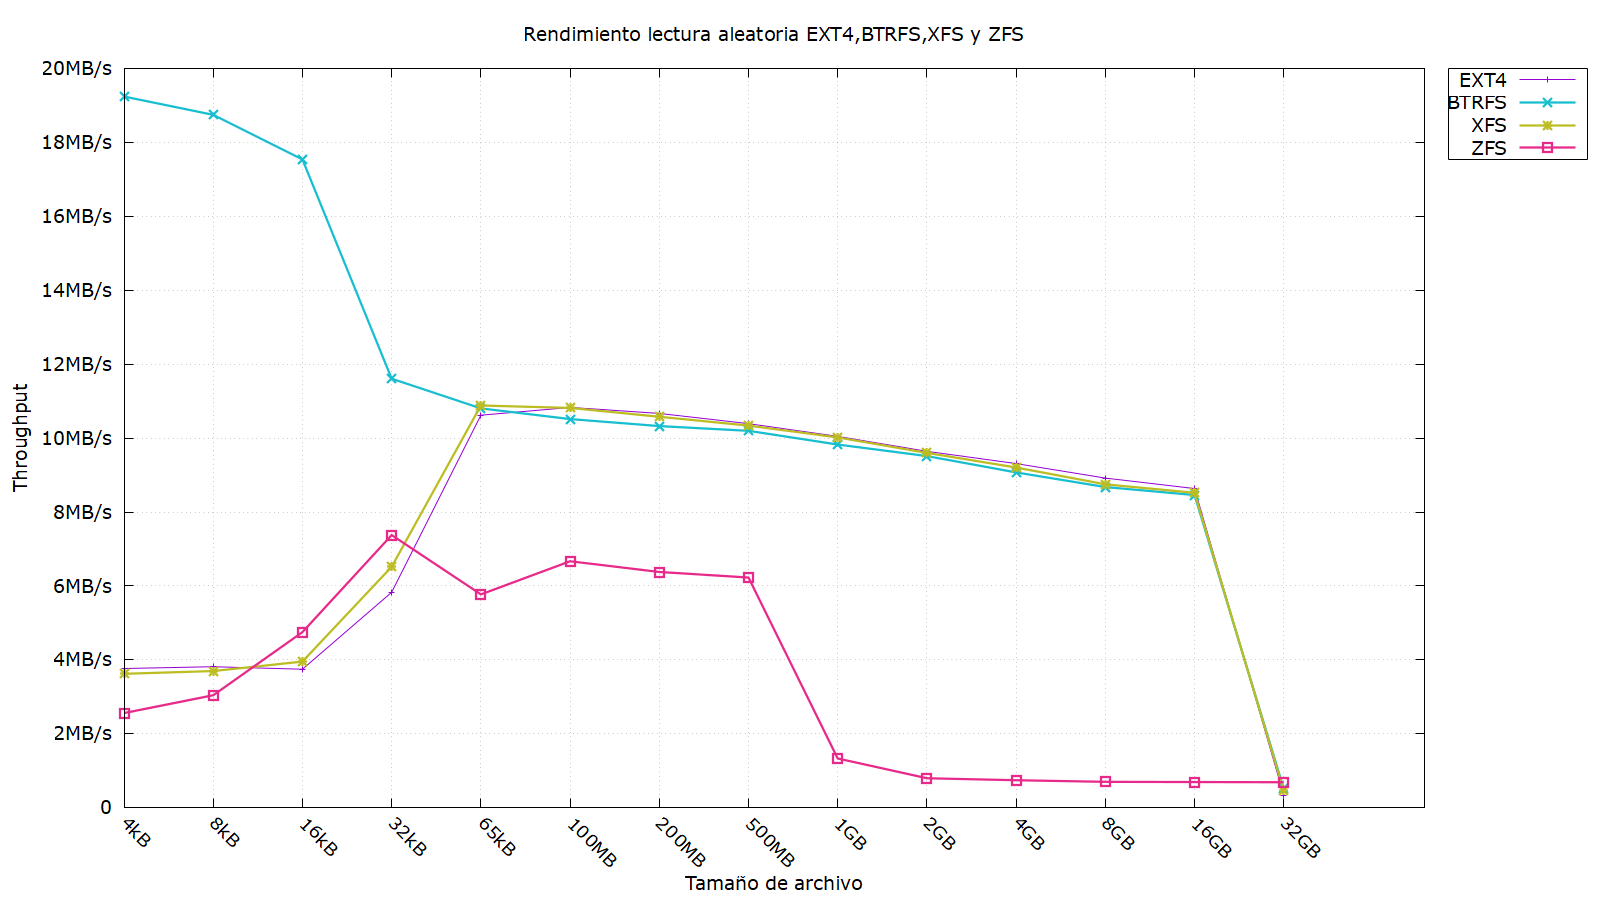
\includegraphics[width=1\linewidth]{results/random_read_throughput_plot.png}
    \caption{Rendimiento de lectura aleatoria de ext4, Btrfs, XFS y ZFS en MB/s}
    \label{fig:lectura_aleatoria_throughput}
\end{figure}

\begin{table}[h!]
\centering
\caption{Rendimiento de lectura aleatoria de ext4, Btrfs, XFS y ZFS en MB/s}
\begin{tabular}{|l|c|c|c|c|}
\hline
\textbf{Métrica} & \textbf{ext4} & \textbf{Btrfs} & \textbf{XFS} & \textbf{ZFS} \\ \hline
Mínimo           & 0,34 MB/s     & 0,51 MB/s      & 0,46 MB/s    & 0,69 MB/s \\ \hline
Máximo           & 10,82 MB/s    & 19,24 MB/s     & 10,88 MB/s   & 7,38 MB/s \\ \hline
Promedio         & 7,61 MB/s     & 11,07 MB/s     & 7,64 MB/s    & 3,41 MB/s \\ \hline
Desviación Típica & 3,42 MB/s     & 4,82 MB/s      & 3,38 MB/s    & 2,66 MB/s \\ \hline
\end{tabular}
\label{tab:rendimiento_lectura_aleatoria_sistemas_archivos}
\end{table}

\newpage

\section{Pruebas de escritura}
\subsection{Escritura}

Una vez más, Btrfs destaca incrementando su rendimiento hasta el tamaño de bloque de 8 kB, debido principalmente a la escritura multisector, que permite enviar las escrituras que son más pequeñas que el tamaño de bloque, en este caso 8 kB, en una sola operación, mejorando significativamente el rendimiento.\\

Además, Btrfs sobresale en los tamaños de fichero pequeños gracias a la implementación de técnicas como la escritura retrasada (delayed write), la compartición de bloques y la escritura coalescente, previamente referenciadas en las características de Btrfs, que optimizan el rendimiento de las escrituras.\\

Ambas técnicas, escritura retrasada y coalescente, son implementadas por Btrfs y explican el rendimiento sobresaliente que obtiene para las escrituras de archivos pequeños. La escritura retrasada permite acumular datos en la caché, y durante ese tiempo, la escritura coalescente puede agrupar estas operaciones en bloques más grandes antes de escribirlos en el disco, maximizando así la eficiencia y el rendimiento.\\

La compartición de bloques en Btrfs también contribuye significativamente a la optimización de las escrituras. Esta técnica permite un uso más eficiente del espacio en disco y reduce la cantidad de escrituras necesarias.\\

Btrfs también se beneficia en la escritura gracias a su estructura interna basada en árboles B+. Las escrituras en una estructura arborescente son mucho más eficientes que las que deben modificar bitmaps, como es el caso de ext4, XFS y ZFS.\\

Podemos observar cómo tanto ext4, Btrfs y XFS presentan caídas pronunciadas en su rendimiento después de alcanzar su pico. Estas caídas se deben principalmente a que la memoria caché se agota, obligando a enviar las peticiones a la cola de disco, lo que causa saturación y un rendimiento reducido.\\

Es notable que ZFS, al igual que en las pruebas anteriores, no alcanza su rendimiento máximo, sino que se mantiene estable a partir de los 200 MB de tamaño de fichero. También es destacable que su rendimiento no decae en los tamaños de fichero más grandes, a diferencia de ext4, Btrfs y XFS. Esto se debe a que ZFS gestiona la caché de manera más eficiente, asegurando la integridad de las operaciones de lectura.\\

Btrfs presenta una caída menos acentuada en comparación con ext4 y XFS, lo cual se atribuye a la mencionada escritura multisector, que agrupa las escrituras y evita que la cola de disco se sature a niveles críticos. \\

\begin{figure}[h!]
    \centering
    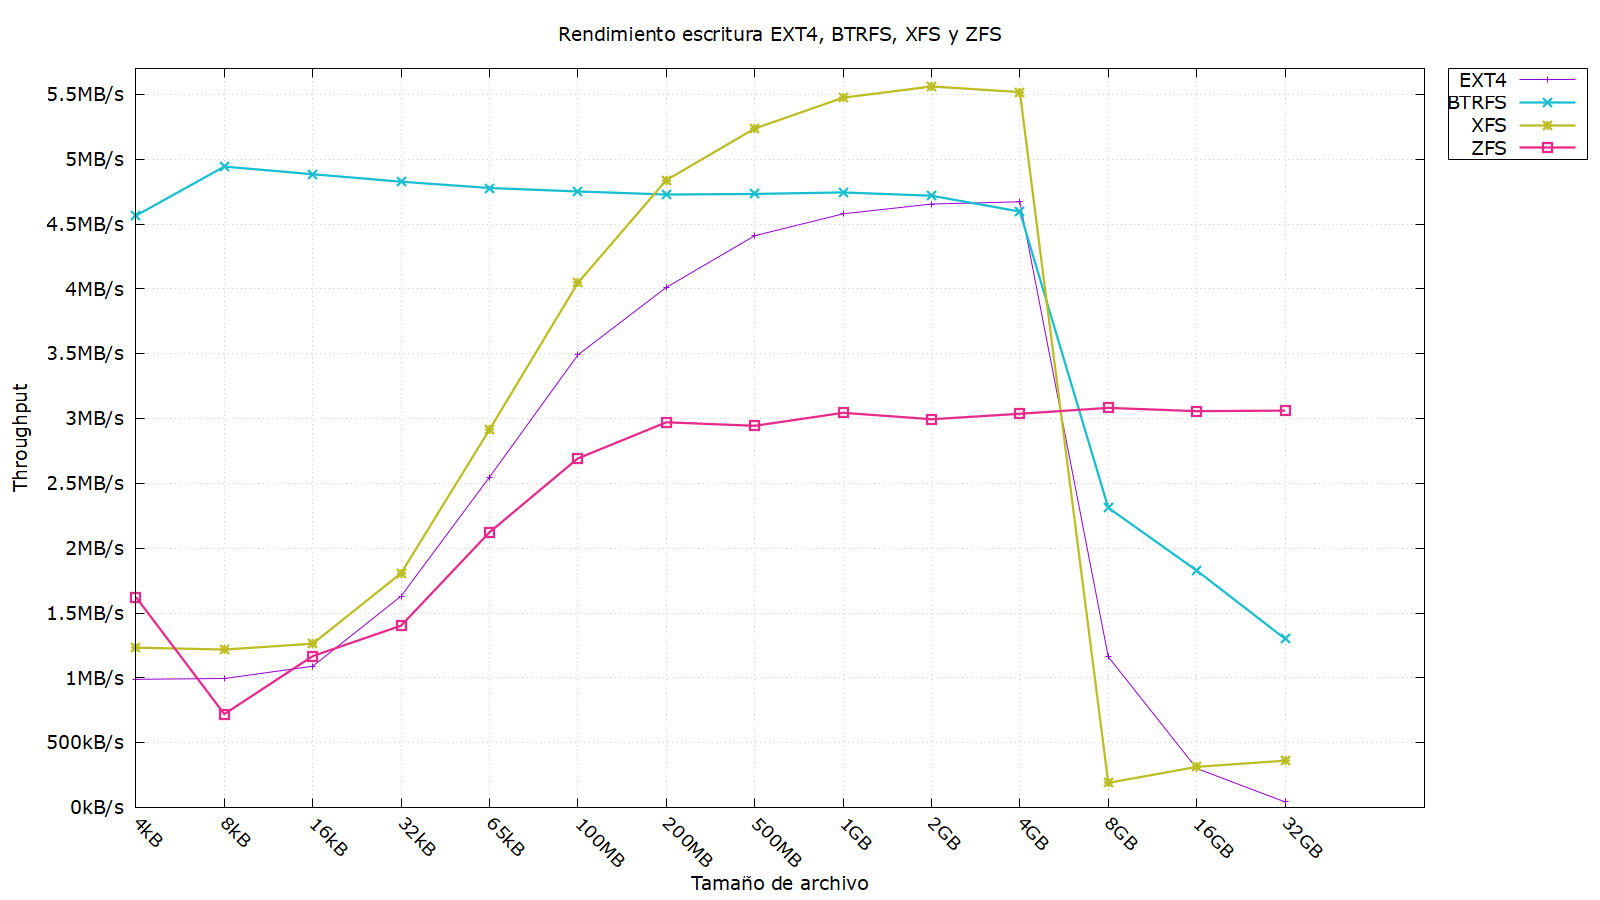
\includegraphics[width=1\linewidth]{results/write_throughput_plot.png}
    \caption{Rendimiento de escritura de ext4, Btrfs, XFS y ZFS en MB/s}
    \label{fig:escritura_throughput}
\end{figure}

\begin{table}[h!]
    \centering
    \caption{Rendimiento de escritura de ext4, Btrfs, XFS y ZFS en MB/s}
    \begin{tabular}{|l|c|c|c|c|}
        \hline
        \textbf{Métrica}  & \textbf{ext4} & \textbf{Btrfs} & \textbf{XFS}  & \textbf{ZFS}  \\ \hline
        Mínimo            & 0,99 MB/s   & 4,57 MB/s   & 1,23 MB/s   & 1,62 MB/s  \\ \hline
        Máximo            & 4,67 MB/s & 4,94 MB/s  & 5,47 MB/s & 3,04 MB/s \\ \hline
        Promedio          & 2,90 MB/s & 4,03 MB/s  & 2,79 MB/s & 2,38 MB/s  \\ \hline
        Desviación Típica & 1,69 MB/s  & 1,31 MB/s   & 2,21 MB/s  & 0,83 MB/s  \\ \hline
    \end{tabular}
    \label{tab:rendimiento_escritura_sistemas_archivos}
\end{table}

En comparación, XFS muestra el mejor rendimiento en las escrituras de archivos grandes, debido principalmente a los grupos de asignación. Los grupos de asignación en XFS permiten que el sistema de archivos gestione sus inodos y espacio libre de forma independiente por cada grupo, posibilitando que múltiples hilos realicen operaciones de escritura simultáneamente sin interferencia, lo que es ideal para aplicaciones que manejan grandes volúmenes de datos.

\subsection{Reescritura}

En el caso de la reescritura, el rendimiento observado supera en todos los casos al de la escritura secuencial, gracias a varios factores clave en la gestión de datos. Primero, no es necesario recrear la tabla de asignación de bloques porque esta ya existe y se mantiene intacta, lo que elimina una operación significativa que consume tiempo. \\

El segundo elemento crucial es la escritura diferida. Normalmente, el intervalo para desencadenar estas escrituras consolidadas es de aproximadamente 30 segundos, aunque puede variar según la configuración del sistema y las circunstancias operativas. Durante operaciones de reescritura, este contador puede retrasarse aún más, reiniciándose si el bloque que se va a escribir aún está en memoria. Esto permite que las operaciones de escritura se agrupen, reduciendo la carga inmediata sobre el disco. \\

Podemos apreciar además que, en el caso de ext4, Btrfs y XFS, es notorio el uso de la escritura diferida. Es importante destacar cómo en este caso, la memoria que el sistema es capaz de dedicar al caché es el limitante, pues como podemos comprobar, una vez el caché está lleno, en el salto de 16GB a 32GB de tamaño de archivo, las escrituras son encoladas al disco, lo que reduce el rendimiento a prácticamente 1MB/s. \\

ZFS, en cambio, presenta un rendimiento estable casi durante toda la prueba, destacándose por no caer en el salto de los 16GB a 32GB de tamaño de fichero. Esto se debe a que la memoria caché realmente no está llena, ya que los algoritmos de compresión e integridad del propio sistema de archivos hacen que las escrituras se envíen a disco y se desalojen páginas del caché. Podríamos decir que, en el caso de este sistema de archivos, los recursos están compartidos de forma equitativa, pues no solo depende de la capacidad del disco para servir a la memoria de bloques, sino que la penalización de la compresión también involucra a la CPU y otros recursos del sistema.

\begin{figure}[h!]
    \centering
    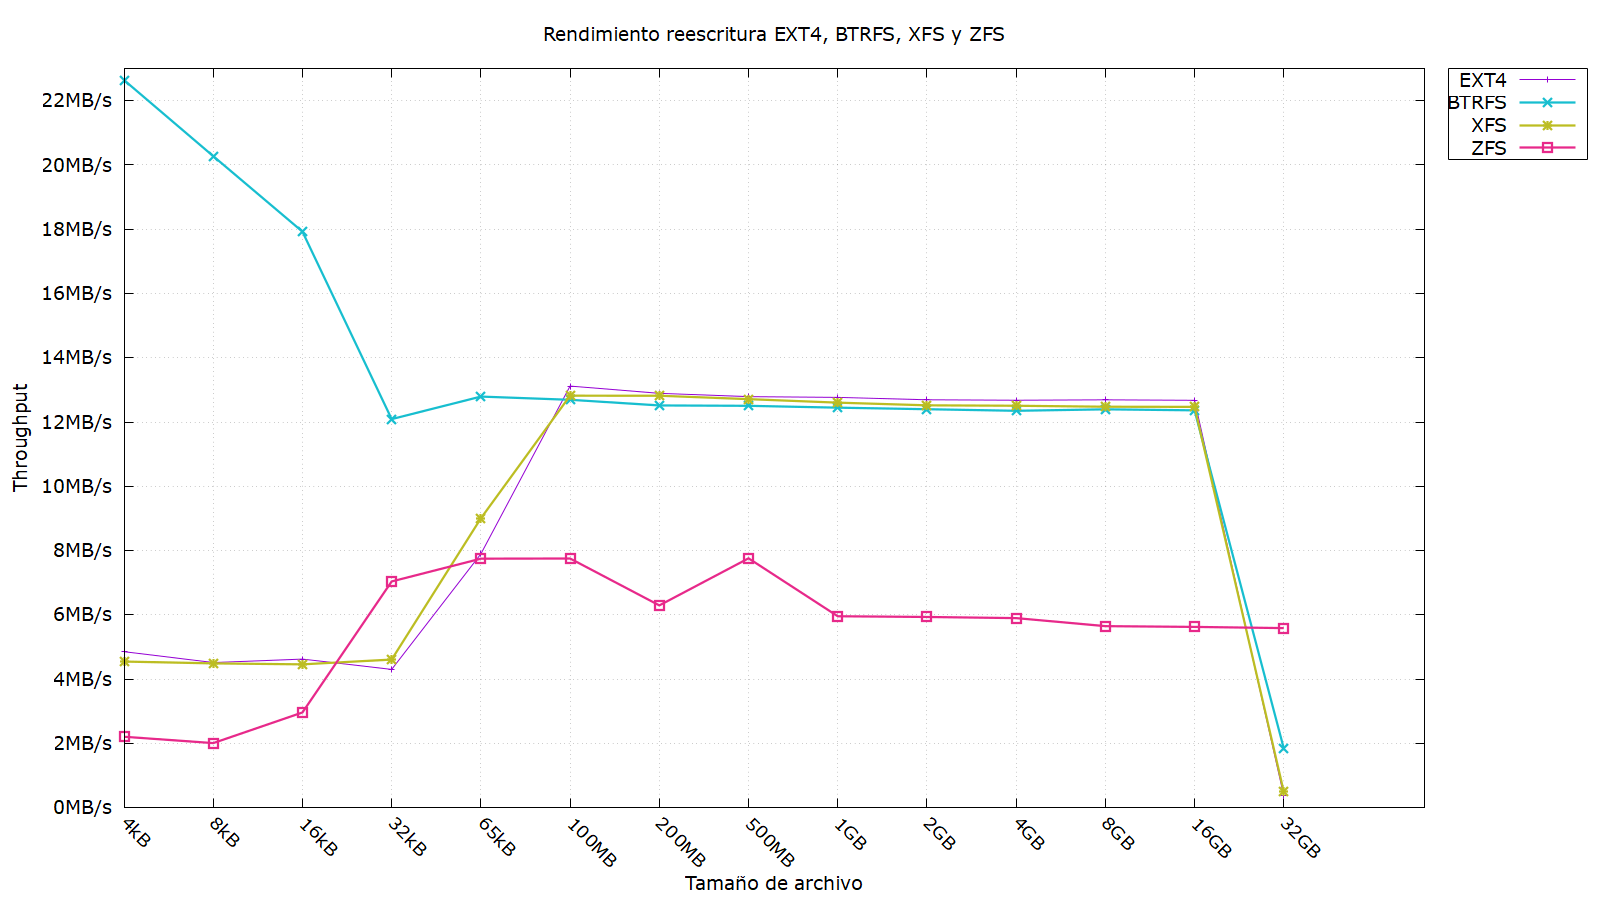
\includegraphics[width=1\linewidth]{results/rewrite_throughput_plot.png}
    \caption{Rendimiento de reescritura de ext4, Btrfs, XFS y ZFS en MB/s}
    \label{fig:reescritura_throughput}
\end{figure}

\begin{table}[h!]
    \centering
    \caption{Rendimiento de reescritura de ext4, Btrfs, XFS y ZFS en MB/s}
    \begin{tabular}{|l|c|c|c|c|}
    \hline
    \textbf{Métrica} & \textbf{ext4} & \textbf{Btrfs} & \textbf{XFS} & \textbf{ZFS} \\ \hline
    Mínimo           & 0,37 MB/s     & 1,85 MB/s      & 0,50 MB/s    & 2,01 MB/s \\ \hline
    Máximo           & 13,12 MB/s    & 22,64 MB/s     & 12,82 MB/s   & 7,76 MB/s \\ \hline
    Promedio         & 9,20 MB/s     & 13,37 MB/s     & 9,18 MB/s    & 5,60 MB/s \\ \hline
    Desviación Típica & 4,55 MB/s    & 4,77 MB/s      & 4,44 MB/s    & 1,92 MB/s \\ \hline
    \end{tabular}
    \label{tab:rendimiento_reescritura_sistemas_archivos}
\end{table}

\subsection{Escritura aleatoria}

Al igual que en las demás escrituras, Btrfs presenta un rendimiento sobresaliente en comparación con otros sistemas de archivos. Esto se debe, como mencionamos previamente, a sus técnicas de escritura diferida, compartición de bloques y escritura coalescente. \\

Podemos observar que, prácticamente desde el comienzo, Btrfs alcanza su rendimiento máximo y, a partir de ahí, su rendimiento disminuye. Esta disminución también afecta a los demás sistemas de archivos y se debe a la propia aleatoriedad intrínseca de la prueba. En otras palabras, perdemos gran parte de la aceleración generada por la caché debido a los numerosos fallos en memoria. Además, esto provoca que la escritura diferida no se vea reseteada y envíe las escrituras al disco de manera anticipada, produciendo un descenso mucho más rápido que en las pruebas anteriores, aproximadamente a partir de los 65 kB. \\

Podemos comprobar también cómo tanto ext4, Btrfs y XFS presentan un rendimiento prácticamente idéntico a partir de los 65 kB, incluso destacando XFS por aproximadamente 0,5 MB en los mejores casos. ZFS, en cambio, sigue la línea de las pruebas anteriores, pero presenta un rendimiento bastante mejor en archivos pequeños, específicamente para 16 kB. \\

\begin{figure}[h!]
    \centering
    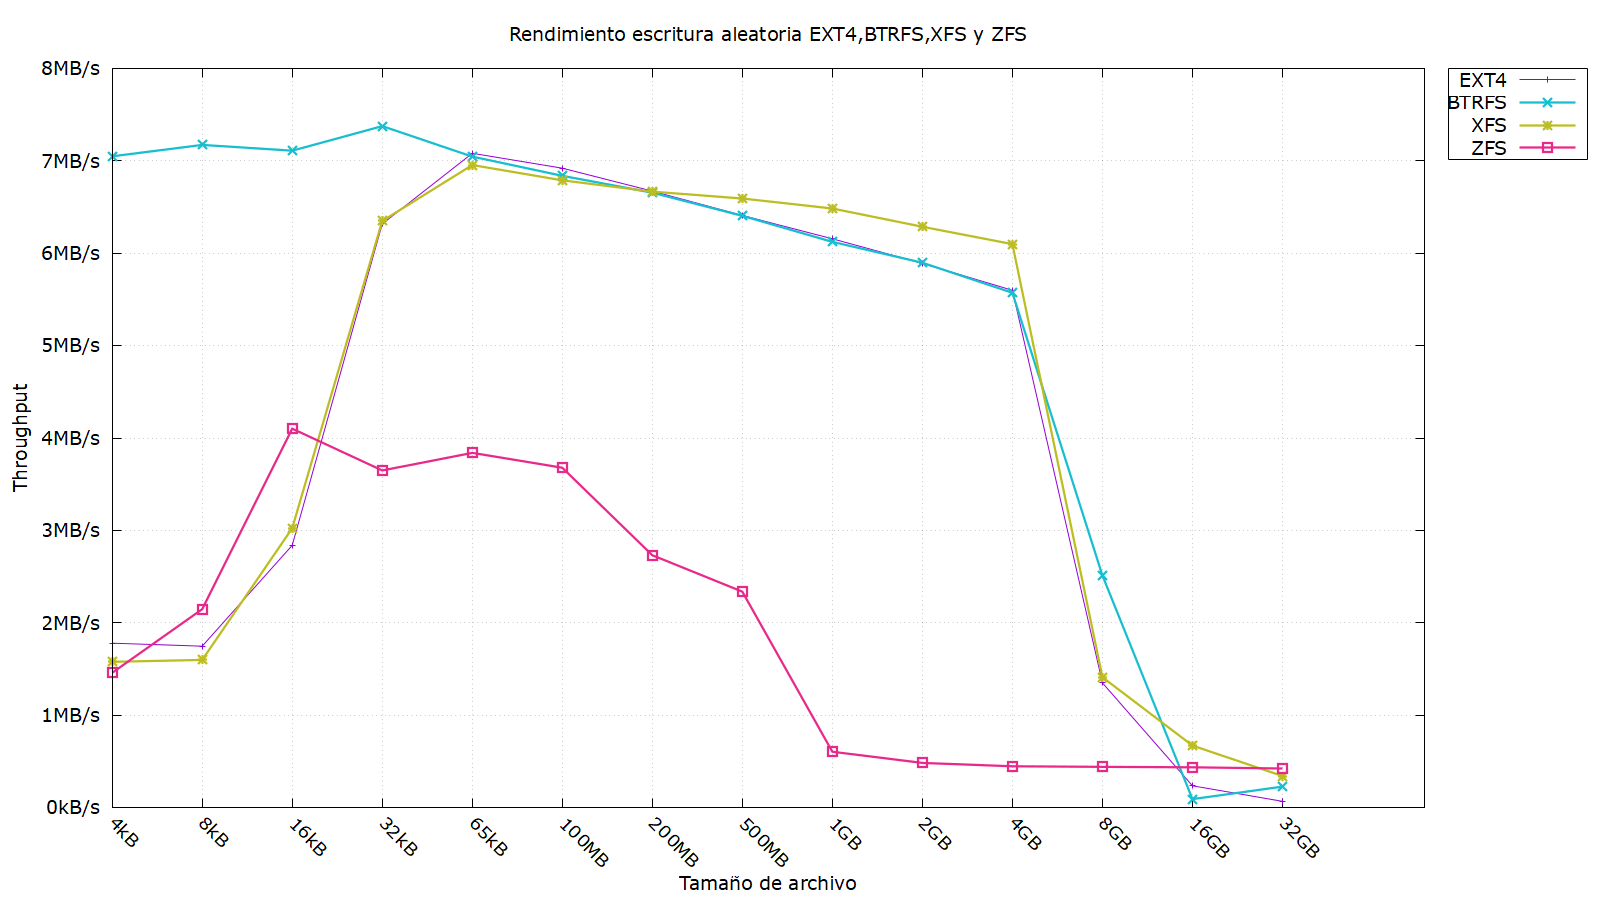
\includegraphics[width=1\linewidth]{results/random_write_throughput_plot.png}
    \caption{Rendimiento de escritura aleatoria de ext4, Btrfs, XFS y ZFS en MB/s}
    \label{fig:escritura_aleatoria_throughput}
\end{figure}

\begin{table}[h!]
\centering
\caption{Rendimiento de escritura aleatoria de ext4, Btrfs, XFS y ZFS en MB/s}
\begin{tabular}{|l|c|c|c|c|}
\hline
\textbf{Métrica} & \textbf{ext4} & \textbf{Btrfs} & \textbf{XFS} & \textbf{ZFS} \\ \hline
Mínimo           & 0,07 MB/s     & 0,09 MB/s      & 0,34 MB/s    & 0,42 MB/s \\ \hline
Máximo           & 7,08 MB/s     & 7,37 MB/s      & 6,96 MB/s    & 4,10 MB/s \\ \hline
Promedio         & 4,22 MB/s     & 5,43 MB/s      & 4,35 MB/s    & 1,91 MB/s \\ \hline
Desviación Típica & 2,70 MB/s     & 2,54 MB/s      & 2,69 MB/s    & 1,47 MB/s \\ \hline
\end{tabular}
\label{tab:rendimiento_escritura_aleatoria_sistemas_archivos}
\end{table}

Encontramos también un descenso abrupto en el rendimiento de Btrfs en la escritura aleatoria, especialmente en archivos pequeños. En este caso, podemos apreciar cómo el rendimiento de ext4, Btrfs y XFS se ve muy afectado por la aleatoriedad de la prueba, produciendo un descenso paulatino conforme el test avanza. Este descenso se debe a la pérdida de gran parte de la aceleración obtenida de la escritura diferida, ya que en este caso la caché se ve obligada a enviar las solicitudes de escritura al disco sin poder agrupar las escrituras coalescentes.





